\documentclass[aspectratio=169,11pt]{beamer}

\usepackage[T1]{fontenc}
\usepackage[utf8]{inputenc}
\usepackage[ngerman]{babel}
\usepackage{graphicx}
\usepackage{lmodern}
\usepackage{booktabs}
\usepackage{xcolor}

\usetheme{Madrid}
\usecolortheme{default}

\definecolor{AccentBlue}{RGB}{21,76,121}
\definecolor{AccentTeal}{RGB}{0,127,140}
\definecolor{AccentGray}{RGB}{74,85,104}

\newcommand{\ProjectName}{DAEDALUS}

\setbeamercolor{structure}{fg=AccentBlue}
\setbeamercolor{title}{fg=white}
\setbeamercolor{frametitle}{fg=white,bg=AccentBlue}
\setbeamercolor{block title}{fg=white,bg=AccentBlue}
\setbeamercolor{block body}{bg=black!3}
\setbeamercolor{itemize item}{fg=AccentTeal}
\setbeamercolor{itemize subitem}{fg=AccentTeal}

\setbeamercolor{headline}{fg=white,bg=AccentBlue}
\setbeamercolor{author in head/foot}{fg=white,bg=AccentBlue}
\setbeamercolor{title in head/foot}{fg=white,bg=AccentBlue}
\setbeamercolor{date in head/foot}{fg=white,bg=AccentBlue}

\setbeamerfont{title}{size=\LARGE,series=\bfseries}
\setbeamerfont{subtitle}{size=\large}
\setbeamerfont{frametitle}{size=\Large,series=\bfseries}
\setbeamerfont{block title}{size=\normalsize,series=\bfseries}
\setbeamerfont{headline}{size=\normalsize,series=\bfseries}

\setbeamertemplate{navigation symbols}{}



\title{6-Achs-3D-Druck mit Robotern}
\subtitle{Projektüberblick zu Medusa, Kronos und Paper}
\author{Adrian Gabriel Axtmann, Ben Stahl, Nik Wachsmann}
\date{14. Mai 2026}

\begin{document}

\begin{frame}[plain]
  \titlepage
\end{frame}

\section{Projektüberblick}
\begin{frame}{Worum geht es und warum ist das spannend?}
  \begin{block}{Projektidee}
    Entwicklung eines prototypischen 6-Achs-Slicer-Stacks für die nichtplanare, robotergestützte additive Fertigung.
  \end{block}

  \begin{columns}[T,totalwidth=\textwidth]
    \begin{column}{0.48\textwidth}
      \begin{block}{Mehrwert des Ansatzes}
        \begin{itemize}
          \item Weg von ebenen Schichten und starrer Z-Achse
          \item Potenzial für weniger Stützstrukturen
          \item Bessere Erreichbarkeit komplexer Geometrien
          \item Stabilere Teile durch Nichtplanarität
        \end{itemize}
      \end{block}
    \end{column}
    \begin{column}{0.48\textwidth}
      \begin{block}{Zwei Bausteine}
        \textbf{Medusa}\\
        Planung und Visualisierung\\[0.7em]
        \textbf{Kronos}\\
        Simulation und Ausführung\\[0.7em]
      \end{block}
    \end{column}
  \end{columns}
\end{frame}

\section{Medusa}
\begin{frame}{Medusa}
  \begin{columns}[T,totalwidth=\textwidth]
    \begin{column}{0.36\textwidth}
      \small
      \raggedright
      \begin{itemize}
        \item Eigene C++-Applikation für Modelle und Druckpfade
        \item Visualisiert Geometrie und exportiert Toolpaths
        \item Sichtbare Planungsseite des Projekts
      \end{itemize}
    \end{column}
    \begin{column}{0.62\textwidth}
      \fbox{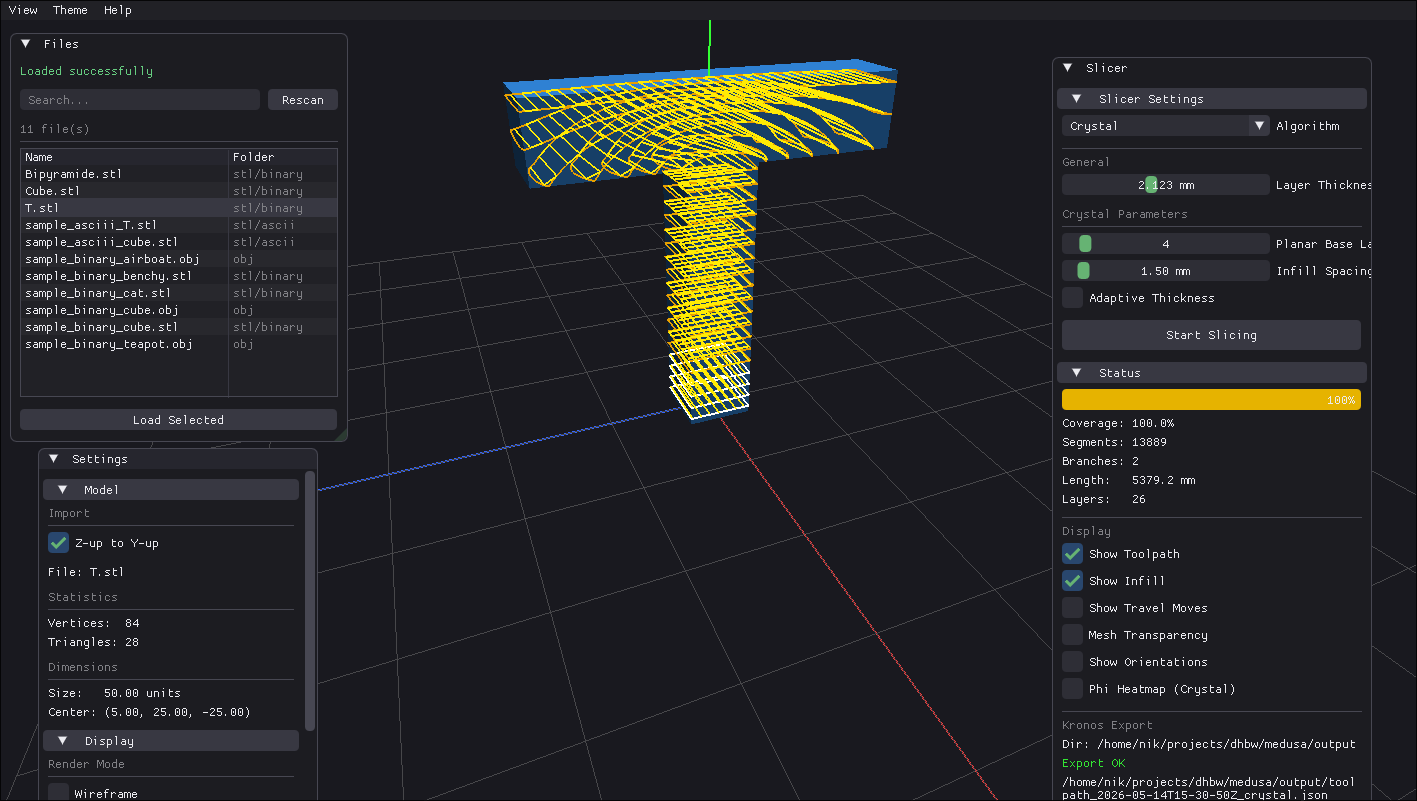
\includegraphics[width=0.94\linewidth,height=4.5cm,keepaspectratio]{MEDUSA.png}}
    \end{column}
  \end{columns}
\end{frame}

\section{Kronos}
\begin{frame}{Kronos}
  \begin{columns}[T,totalwidth=\textwidth]
    \begin{column}{0.36\textwidth}
      \small
      \raggedright
      \begin{itemize}
        \item ROS-2- und MoveIt-Umgebung für den UR3e
        \item Liest Toolpaths ein und plant Roboterbewegungen
        \item Bringt die Planung in die Simulation
      \end{itemize}
    \end{column}
    \begin{column}{0.62\textwidth}
      \fbox{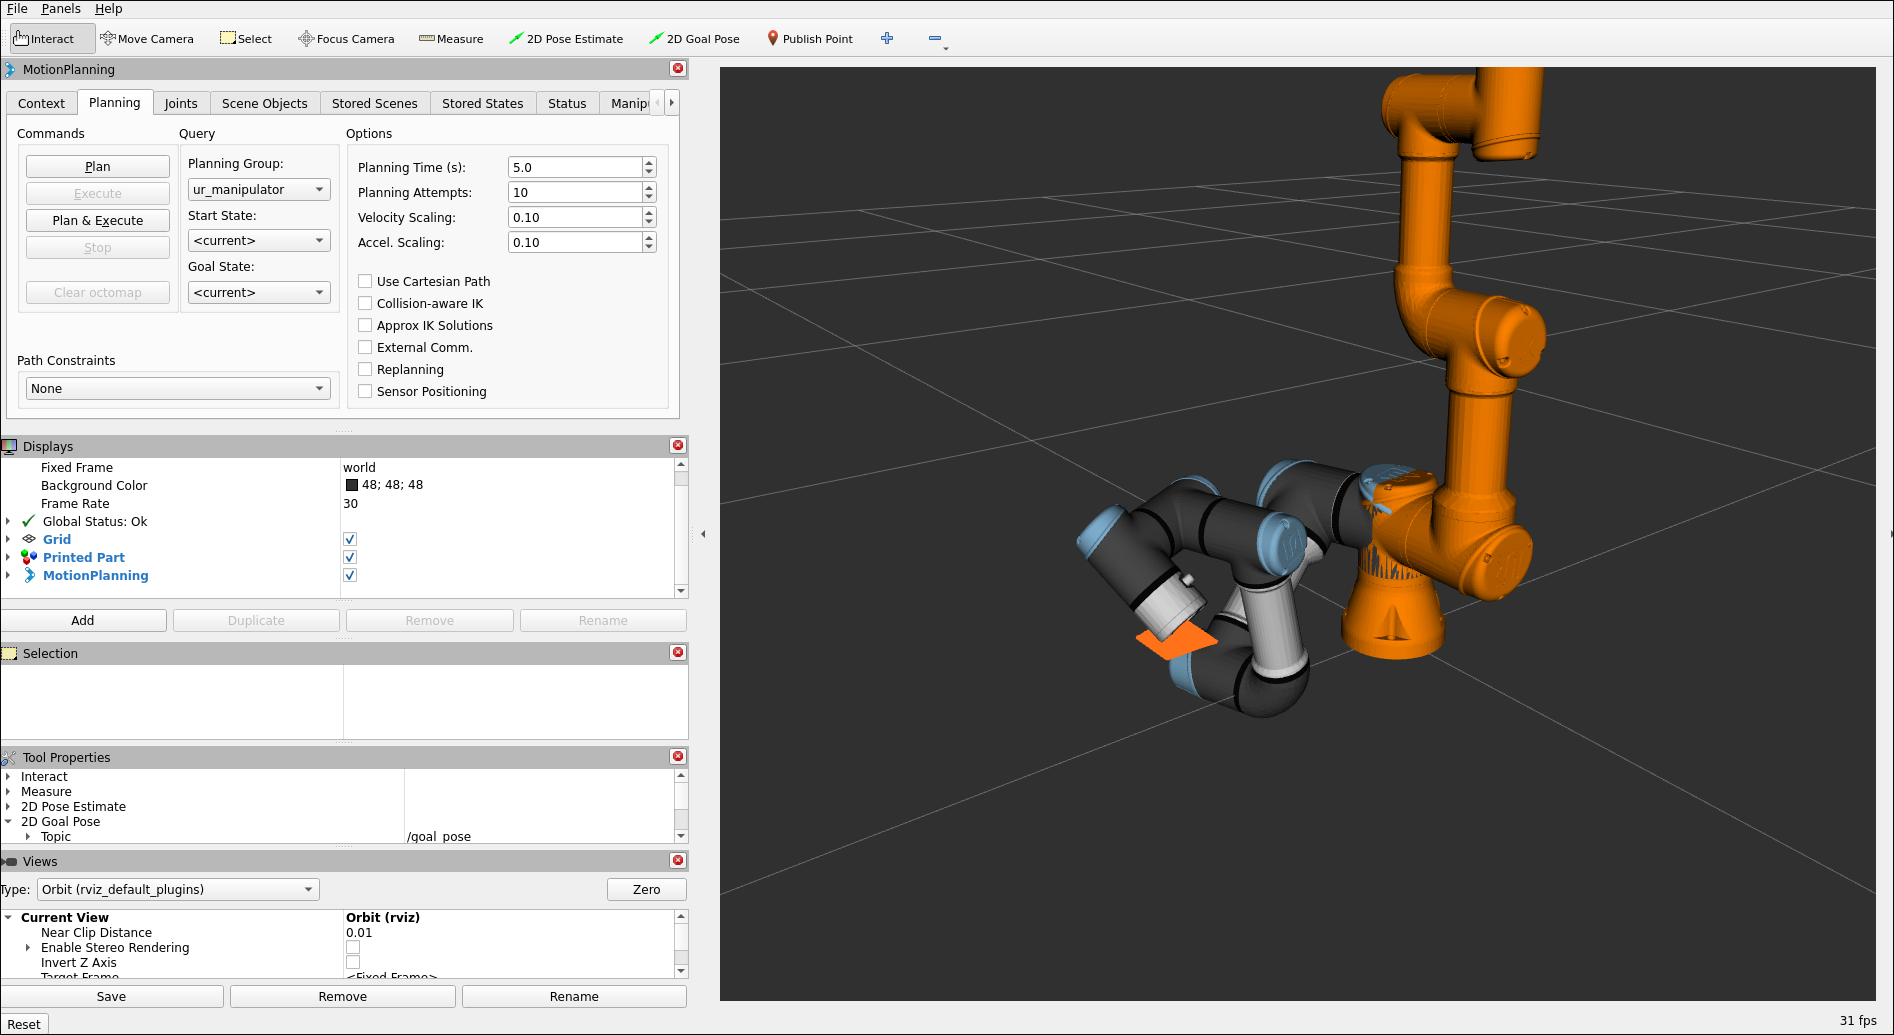
\includegraphics[width=0.94\linewidth,height=4.5cm,keepaspectratio]{KRONOS.png}}
    \end{column}
  \end{columns}
\end{frame}

\section{Ausblick}
\begin{frame}{Projektstand und Ausblick}
  \begin{block}{Aktueller Mehrwert}
    Sichtbarer Prototyp von der Modellverarbeitung bis zur Roboter-Validierung.
  \end{block}

  \begin{itemize}
    \item Verbindet Softwareentwicklung, Robotik und additive Fertigung
    \item Fokus ist das nichtplanare Slicing, nicht das physische Drucken
  \end{itemize}
\end{frame}

\end{document}